% Generated by Sphinx.
\def\sphinxdocclass{report}
\documentclass[letterpaper,10pt,english]{sphinxmanual}
\usepackage[utf8]{inputenc}
\DeclareUnicodeCharacter{00A0}{\nobreakspace}
\usepackage{cmap}
\usepackage[T1]{fontenc}
\usepackage{babel}
\usepackage{times}
\usepackage[Bjarne]{fncychap}
\usepackage{longtable}
\usepackage{sphinx}
\usepackage{multirow}


\title{sentinelSimulator Documentation}
\date{August 11, 2017}
\release{0.0.1}
\author{E. Pinnington}
\newcommand{\sphinxlogo}{}
\renewcommand{\releasename}{Release}
\makeindex

\makeatletter
\def\PYG@reset{\let\PYG@it=\relax \let\PYG@bf=\relax%
    \let\PYG@ul=\relax \let\PYG@tc=\relax%
    \let\PYG@bc=\relax \let\PYG@ff=\relax}
\def\PYG@tok#1{\csname PYG@tok@#1\endcsname}
\def\PYG@toks#1+{\ifx\relax#1\empty\else%
    \PYG@tok{#1}\expandafter\PYG@toks\fi}
\def\PYG@do#1{\PYG@bc{\PYG@tc{\PYG@ul{%
    \PYG@it{\PYG@bf{\PYG@ff{#1}}}}}}}
\def\PYG#1#2{\PYG@reset\PYG@toks#1+\relax+\PYG@do{#2}}

\expandafter\def\csname PYG@tok@gd\endcsname{\def\PYG@tc##1{\textcolor[rgb]{0.63,0.00,0.00}{##1}}}
\expandafter\def\csname PYG@tok@gu\endcsname{\let\PYG@bf=\textbf\def\PYG@tc##1{\textcolor[rgb]{0.50,0.00,0.50}{##1}}}
\expandafter\def\csname PYG@tok@gt\endcsname{\def\PYG@tc##1{\textcolor[rgb]{0.00,0.27,0.87}{##1}}}
\expandafter\def\csname PYG@tok@gs\endcsname{\let\PYG@bf=\textbf}
\expandafter\def\csname PYG@tok@gr\endcsname{\def\PYG@tc##1{\textcolor[rgb]{1.00,0.00,0.00}{##1}}}
\expandafter\def\csname PYG@tok@cm\endcsname{\let\PYG@it=\textit\def\PYG@tc##1{\textcolor[rgb]{0.25,0.50,0.56}{##1}}}
\expandafter\def\csname PYG@tok@vg\endcsname{\def\PYG@tc##1{\textcolor[rgb]{0.73,0.38,0.84}{##1}}}
\expandafter\def\csname PYG@tok@vi\endcsname{\def\PYG@tc##1{\textcolor[rgb]{0.73,0.38,0.84}{##1}}}
\expandafter\def\csname PYG@tok@mh\endcsname{\def\PYG@tc##1{\textcolor[rgb]{0.13,0.50,0.31}{##1}}}
\expandafter\def\csname PYG@tok@cs\endcsname{\def\PYG@tc##1{\textcolor[rgb]{0.25,0.50,0.56}{##1}}\def\PYG@bc##1{\setlength{\fboxsep}{0pt}\colorbox[rgb]{1.00,0.94,0.94}{\strut ##1}}}
\expandafter\def\csname PYG@tok@ge\endcsname{\let\PYG@it=\textit}
\expandafter\def\csname PYG@tok@vc\endcsname{\def\PYG@tc##1{\textcolor[rgb]{0.73,0.38,0.84}{##1}}}
\expandafter\def\csname PYG@tok@il\endcsname{\def\PYG@tc##1{\textcolor[rgb]{0.13,0.50,0.31}{##1}}}
\expandafter\def\csname PYG@tok@go\endcsname{\def\PYG@tc##1{\textcolor[rgb]{0.20,0.20,0.20}{##1}}}
\expandafter\def\csname PYG@tok@cp\endcsname{\def\PYG@tc##1{\textcolor[rgb]{0.00,0.44,0.13}{##1}}}
\expandafter\def\csname PYG@tok@gi\endcsname{\def\PYG@tc##1{\textcolor[rgb]{0.00,0.63,0.00}{##1}}}
\expandafter\def\csname PYG@tok@gh\endcsname{\let\PYG@bf=\textbf\def\PYG@tc##1{\textcolor[rgb]{0.00,0.00,0.50}{##1}}}
\expandafter\def\csname PYG@tok@ni\endcsname{\let\PYG@bf=\textbf\def\PYG@tc##1{\textcolor[rgb]{0.84,0.33,0.22}{##1}}}
\expandafter\def\csname PYG@tok@nl\endcsname{\let\PYG@bf=\textbf\def\PYG@tc##1{\textcolor[rgb]{0.00,0.13,0.44}{##1}}}
\expandafter\def\csname PYG@tok@nn\endcsname{\let\PYG@bf=\textbf\def\PYG@tc##1{\textcolor[rgb]{0.05,0.52,0.71}{##1}}}
\expandafter\def\csname PYG@tok@no\endcsname{\def\PYG@tc##1{\textcolor[rgb]{0.38,0.68,0.84}{##1}}}
\expandafter\def\csname PYG@tok@na\endcsname{\def\PYG@tc##1{\textcolor[rgb]{0.25,0.44,0.63}{##1}}}
\expandafter\def\csname PYG@tok@nb\endcsname{\def\PYG@tc##1{\textcolor[rgb]{0.00,0.44,0.13}{##1}}}
\expandafter\def\csname PYG@tok@nc\endcsname{\let\PYG@bf=\textbf\def\PYG@tc##1{\textcolor[rgb]{0.05,0.52,0.71}{##1}}}
\expandafter\def\csname PYG@tok@nd\endcsname{\let\PYG@bf=\textbf\def\PYG@tc##1{\textcolor[rgb]{0.33,0.33,0.33}{##1}}}
\expandafter\def\csname PYG@tok@ne\endcsname{\def\PYG@tc##1{\textcolor[rgb]{0.00,0.44,0.13}{##1}}}
\expandafter\def\csname PYG@tok@nf\endcsname{\def\PYG@tc##1{\textcolor[rgb]{0.02,0.16,0.49}{##1}}}
\expandafter\def\csname PYG@tok@si\endcsname{\let\PYG@it=\textit\def\PYG@tc##1{\textcolor[rgb]{0.44,0.63,0.82}{##1}}}
\expandafter\def\csname PYG@tok@s2\endcsname{\def\PYG@tc##1{\textcolor[rgb]{0.25,0.44,0.63}{##1}}}
\expandafter\def\csname PYG@tok@nt\endcsname{\let\PYG@bf=\textbf\def\PYG@tc##1{\textcolor[rgb]{0.02,0.16,0.45}{##1}}}
\expandafter\def\csname PYG@tok@nv\endcsname{\def\PYG@tc##1{\textcolor[rgb]{0.73,0.38,0.84}{##1}}}
\expandafter\def\csname PYG@tok@s1\endcsname{\def\PYG@tc##1{\textcolor[rgb]{0.25,0.44,0.63}{##1}}}
\expandafter\def\csname PYG@tok@ch\endcsname{\let\PYG@it=\textit\def\PYG@tc##1{\textcolor[rgb]{0.25,0.50,0.56}{##1}}}
\expandafter\def\csname PYG@tok@m\endcsname{\def\PYG@tc##1{\textcolor[rgb]{0.13,0.50,0.31}{##1}}}
\expandafter\def\csname PYG@tok@gp\endcsname{\let\PYG@bf=\textbf\def\PYG@tc##1{\textcolor[rgb]{0.78,0.36,0.04}{##1}}}
\expandafter\def\csname PYG@tok@sh\endcsname{\def\PYG@tc##1{\textcolor[rgb]{0.25,0.44,0.63}{##1}}}
\expandafter\def\csname PYG@tok@ow\endcsname{\let\PYG@bf=\textbf\def\PYG@tc##1{\textcolor[rgb]{0.00,0.44,0.13}{##1}}}
\expandafter\def\csname PYG@tok@sx\endcsname{\def\PYG@tc##1{\textcolor[rgb]{0.78,0.36,0.04}{##1}}}
\expandafter\def\csname PYG@tok@bp\endcsname{\def\PYG@tc##1{\textcolor[rgb]{0.00,0.44,0.13}{##1}}}
\expandafter\def\csname PYG@tok@c1\endcsname{\let\PYG@it=\textit\def\PYG@tc##1{\textcolor[rgb]{0.25,0.50,0.56}{##1}}}
\expandafter\def\csname PYG@tok@o\endcsname{\def\PYG@tc##1{\textcolor[rgb]{0.40,0.40,0.40}{##1}}}
\expandafter\def\csname PYG@tok@kc\endcsname{\let\PYG@bf=\textbf\def\PYG@tc##1{\textcolor[rgb]{0.00,0.44,0.13}{##1}}}
\expandafter\def\csname PYG@tok@c\endcsname{\let\PYG@it=\textit\def\PYG@tc##1{\textcolor[rgb]{0.25,0.50,0.56}{##1}}}
\expandafter\def\csname PYG@tok@mf\endcsname{\def\PYG@tc##1{\textcolor[rgb]{0.13,0.50,0.31}{##1}}}
\expandafter\def\csname PYG@tok@err\endcsname{\def\PYG@bc##1{\setlength{\fboxsep}{0pt}\fcolorbox[rgb]{1.00,0.00,0.00}{1,1,1}{\strut ##1}}}
\expandafter\def\csname PYG@tok@mb\endcsname{\def\PYG@tc##1{\textcolor[rgb]{0.13,0.50,0.31}{##1}}}
\expandafter\def\csname PYG@tok@ss\endcsname{\def\PYG@tc##1{\textcolor[rgb]{0.32,0.47,0.09}{##1}}}
\expandafter\def\csname PYG@tok@sr\endcsname{\def\PYG@tc##1{\textcolor[rgb]{0.14,0.33,0.53}{##1}}}
\expandafter\def\csname PYG@tok@mo\endcsname{\def\PYG@tc##1{\textcolor[rgb]{0.13,0.50,0.31}{##1}}}
\expandafter\def\csname PYG@tok@kd\endcsname{\let\PYG@bf=\textbf\def\PYG@tc##1{\textcolor[rgb]{0.00,0.44,0.13}{##1}}}
\expandafter\def\csname PYG@tok@mi\endcsname{\def\PYG@tc##1{\textcolor[rgb]{0.13,0.50,0.31}{##1}}}
\expandafter\def\csname PYG@tok@kn\endcsname{\let\PYG@bf=\textbf\def\PYG@tc##1{\textcolor[rgb]{0.00,0.44,0.13}{##1}}}
\expandafter\def\csname PYG@tok@cpf\endcsname{\let\PYG@it=\textit\def\PYG@tc##1{\textcolor[rgb]{0.25,0.50,0.56}{##1}}}
\expandafter\def\csname PYG@tok@kr\endcsname{\let\PYG@bf=\textbf\def\PYG@tc##1{\textcolor[rgb]{0.00,0.44,0.13}{##1}}}
\expandafter\def\csname PYG@tok@s\endcsname{\def\PYG@tc##1{\textcolor[rgb]{0.25,0.44,0.63}{##1}}}
\expandafter\def\csname PYG@tok@kp\endcsname{\def\PYG@tc##1{\textcolor[rgb]{0.00,0.44,0.13}{##1}}}
\expandafter\def\csname PYG@tok@w\endcsname{\def\PYG@tc##1{\textcolor[rgb]{0.73,0.73,0.73}{##1}}}
\expandafter\def\csname PYG@tok@kt\endcsname{\def\PYG@tc##1{\textcolor[rgb]{0.56,0.13,0.00}{##1}}}
\expandafter\def\csname PYG@tok@sc\endcsname{\def\PYG@tc##1{\textcolor[rgb]{0.25,0.44,0.63}{##1}}}
\expandafter\def\csname PYG@tok@sb\endcsname{\def\PYG@tc##1{\textcolor[rgb]{0.25,0.44,0.63}{##1}}}
\expandafter\def\csname PYG@tok@k\endcsname{\let\PYG@bf=\textbf\def\PYG@tc##1{\textcolor[rgb]{0.00,0.44,0.13}{##1}}}
\expandafter\def\csname PYG@tok@se\endcsname{\let\PYG@bf=\textbf\def\PYG@tc##1{\textcolor[rgb]{0.25,0.44,0.63}{##1}}}
\expandafter\def\csname PYG@tok@sd\endcsname{\let\PYG@it=\textit\def\PYG@tc##1{\textcolor[rgb]{0.25,0.44,0.63}{##1}}}

\def\PYGZbs{\char`\\}
\def\PYGZus{\char`\_}
\def\PYGZob{\char`\{}
\def\PYGZcb{\char`\}}
\def\PYGZca{\char`\^}
\def\PYGZam{\char`\&}
\def\PYGZlt{\char`\<}
\def\PYGZgt{\char`\>}
\def\PYGZsh{\char`\#}
\def\PYGZpc{\char`\%}
\def\PYGZdl{\char`\$}
\def\PYGZhy{\char`\-}
\def\PYGZsq{\char`\'}
\def\PYGZdq{\char`\"}
\def\PYGZti{\char`\~}
% for compatibility with earlier versions
\def\PYGZat{@}
\def\PYGZlb{[}
\def\PYGZrb{]}
\makeatother

\begin{document}

\maketitle
\tableofcontents
\phantomsection\label{index::doc}



\chapter{Contents:}
\label{index:welcome-to-sentinelsimulator-s-documentation}\label{index:contents}

\section{sentinelSimulator}
\label{source/README::doc}\label{source/README:sentinelsimulator}
This Python package simulates Sentinel 2 data based on output from the JULES land surface model. Here we provide
documentation on this package. Below we illustrate a basic explanation of the package in use.

Example of using sentinelSimulator package:

\begin{Verbatim}[commandchars=\\\{\}]
\PYG{k+kn}{import} \PYG{n+nn}{simulator} \PYG{k+kn}{as} \PYG{n+nn}{sim}
\PYG{c+c1}{\PYGZsh{} Create class instance containing sentinel simulator data}
\PYG{n}{sim}\PYG{o}{.}\PYG{n}{Simulator}\PYG{p}{(}\PYG{n}{year}\PYG{o}{=}\PYG{l+m+mi}{2012}\PYG{p}{,} \PYG{n}{month}\PYG{o}{=}\PYG{l+m+mi}{1}\PYG{p}{,} \PYG{n}{days}\PYG{o}{=}\PYG{l+m+mi}{365}\PYG{p}{)}
\end{Verbatim}


\subsection{Features}
\label{source/README:features}\begin{itemize}
\item {} 
Simulates sentinel 2 data from JULES output

\item {} 
Add additional explanation

\end{itemize}


\subsection{Source Code}
\label{source/README:source-code}
github.com/example\_user/sentinelSimulator


\subsection{Support}
\label{source/README:support}
If you are having issues, please let us know.
Contact: \href{mailto:ewan.pinnington@gmail.com}{ewan.pinnington@gmail.com}


\subsection{License}
\label{source/README:license}
Details of licensing information.


\section{Example Output}
\label{source/example::doc}\label{source/example:example-output}
Here we show some example output from the Sentinel simulator.

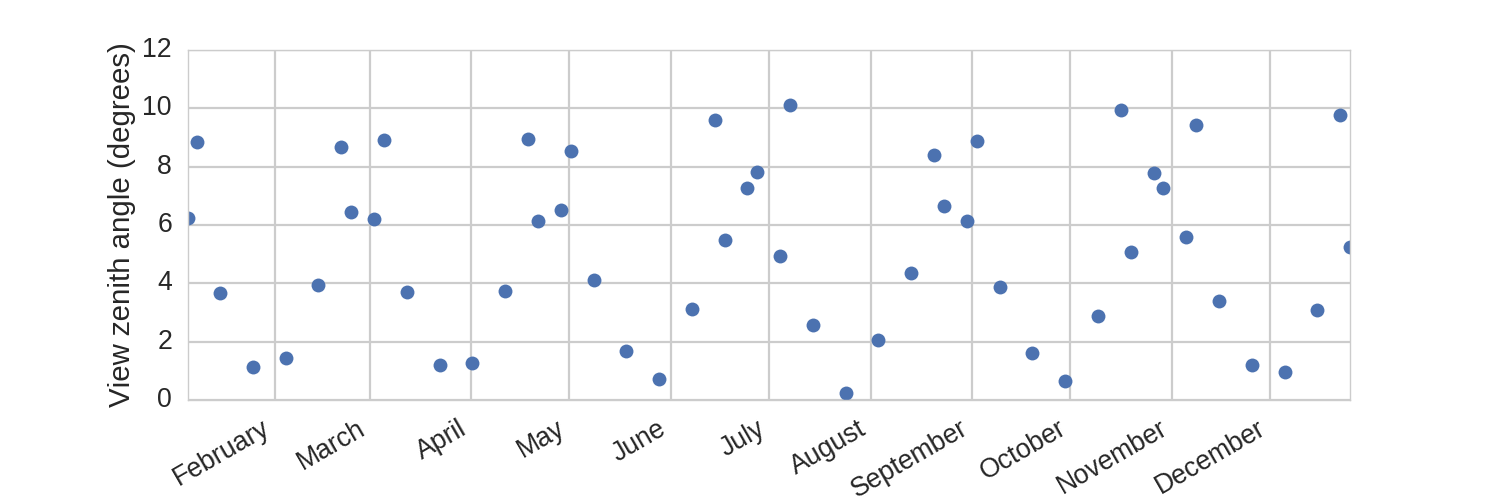
\includegraphics{vza.png}

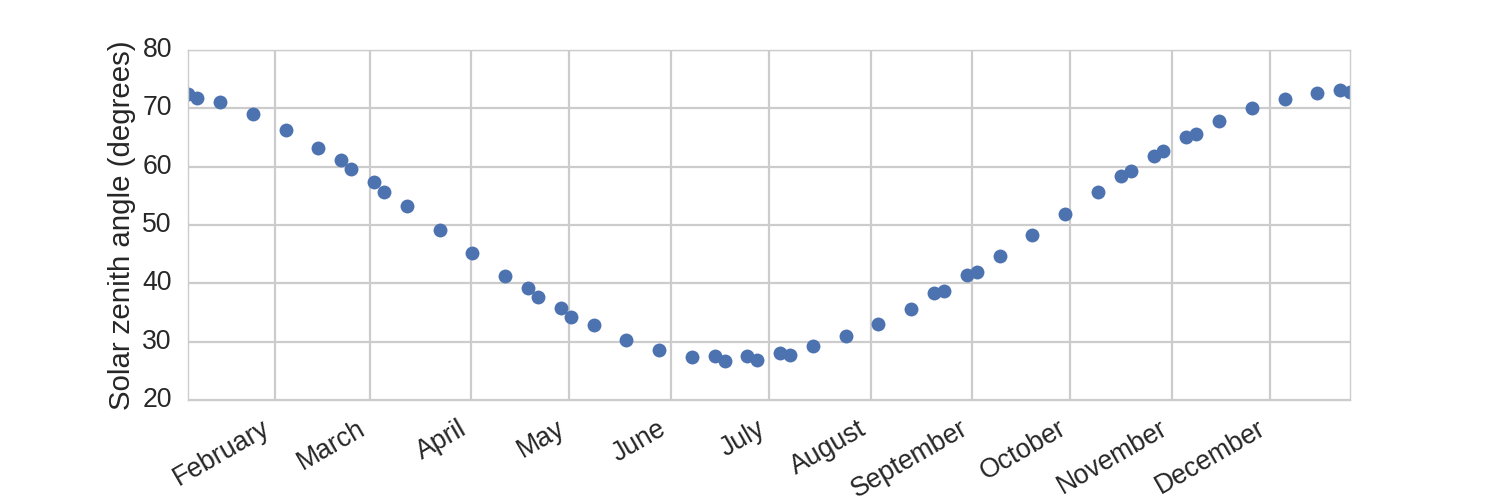
\includegraphics{sza.png}

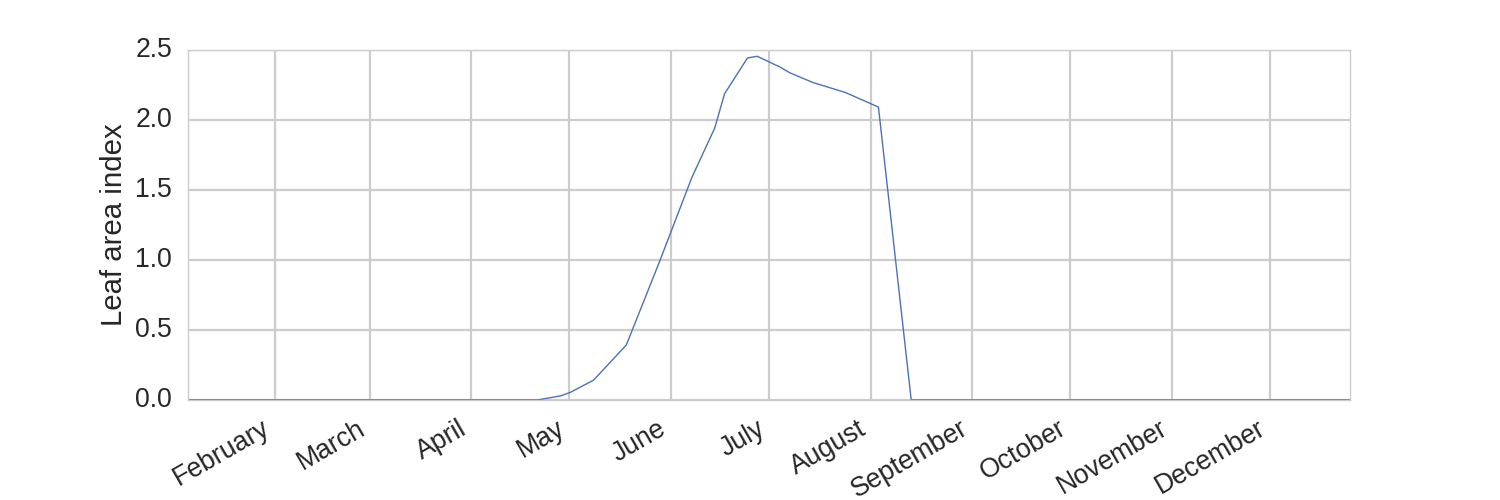
\includegraphics{lai.png}

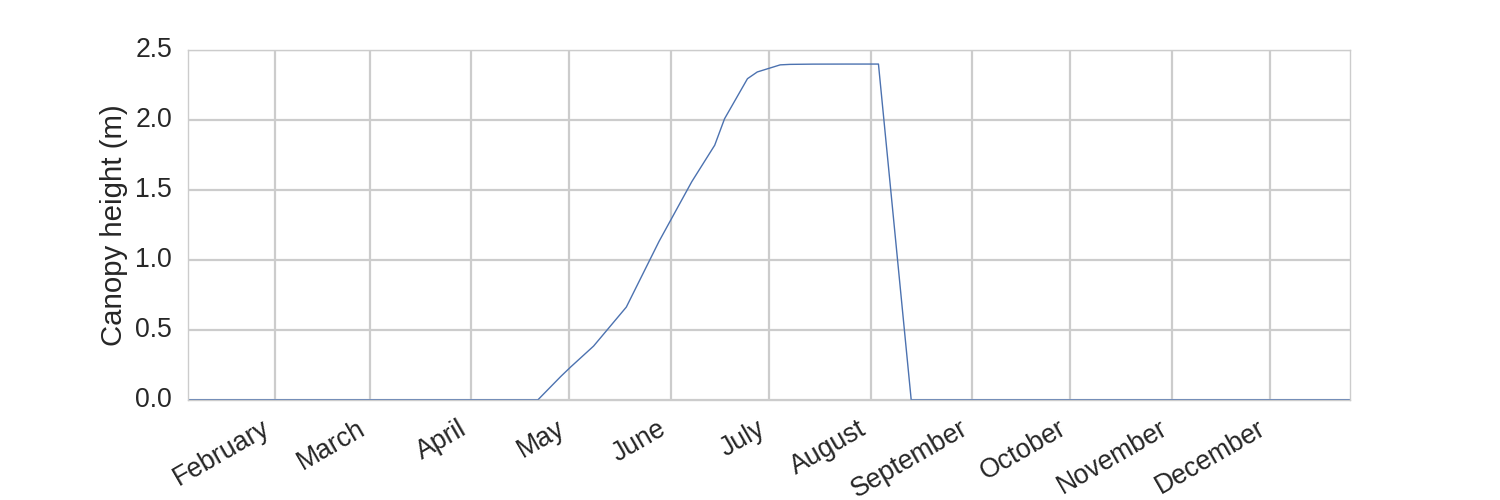
\includegraphics{can_ht.png}

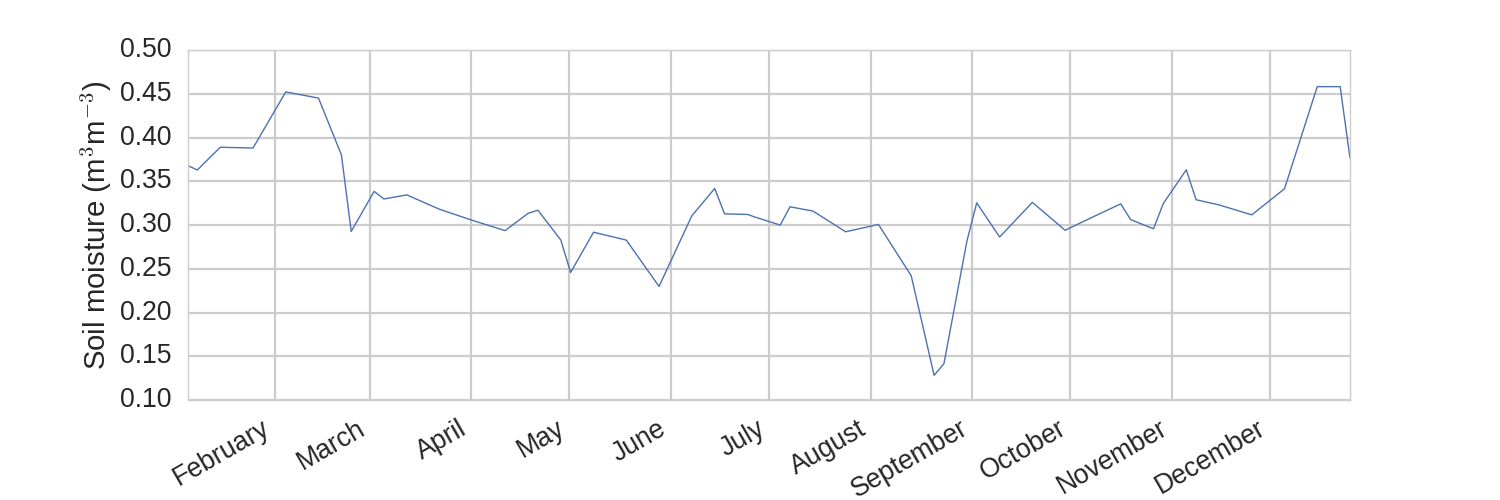
\includegraphics{soil_m.png}

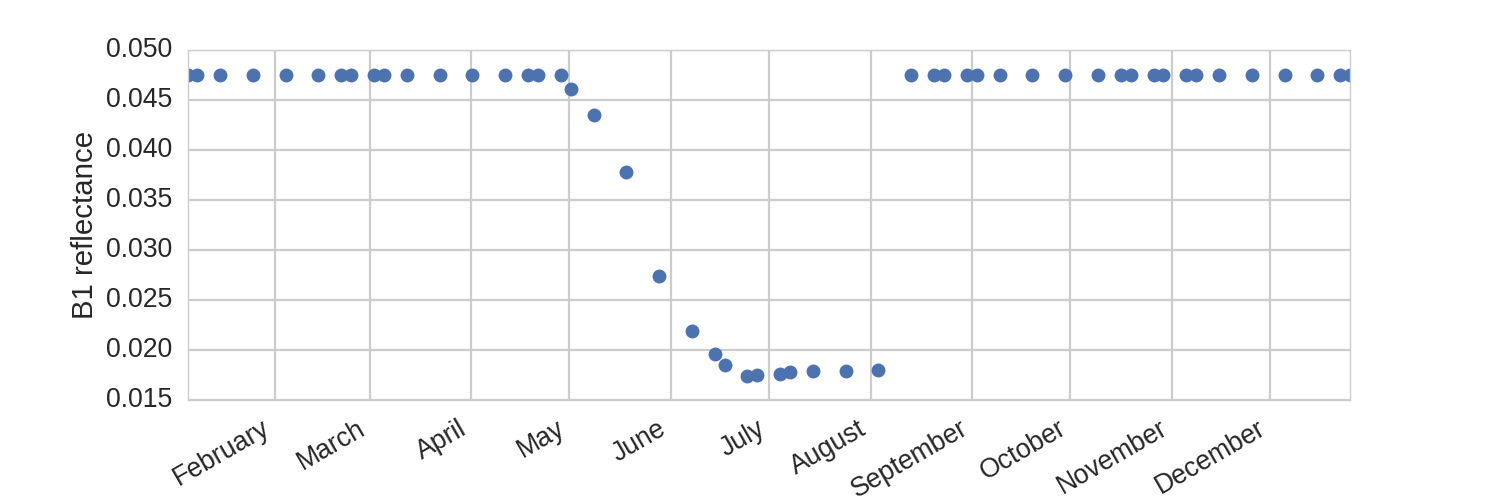
\includegraphics{B1.png}

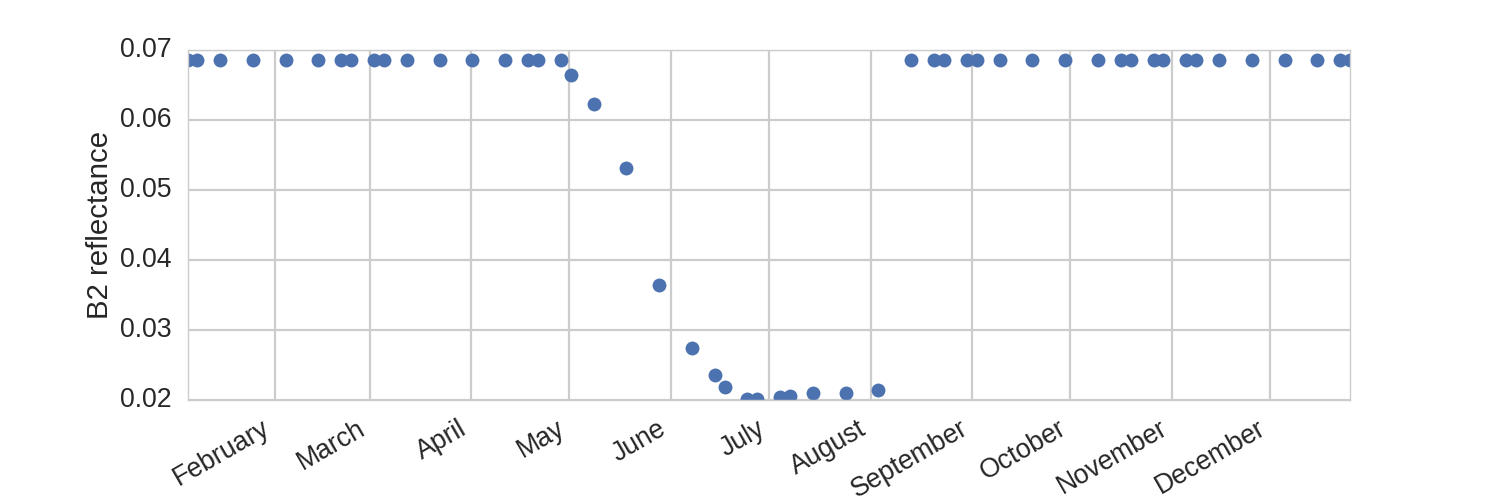
\includegraphics{B2.png}

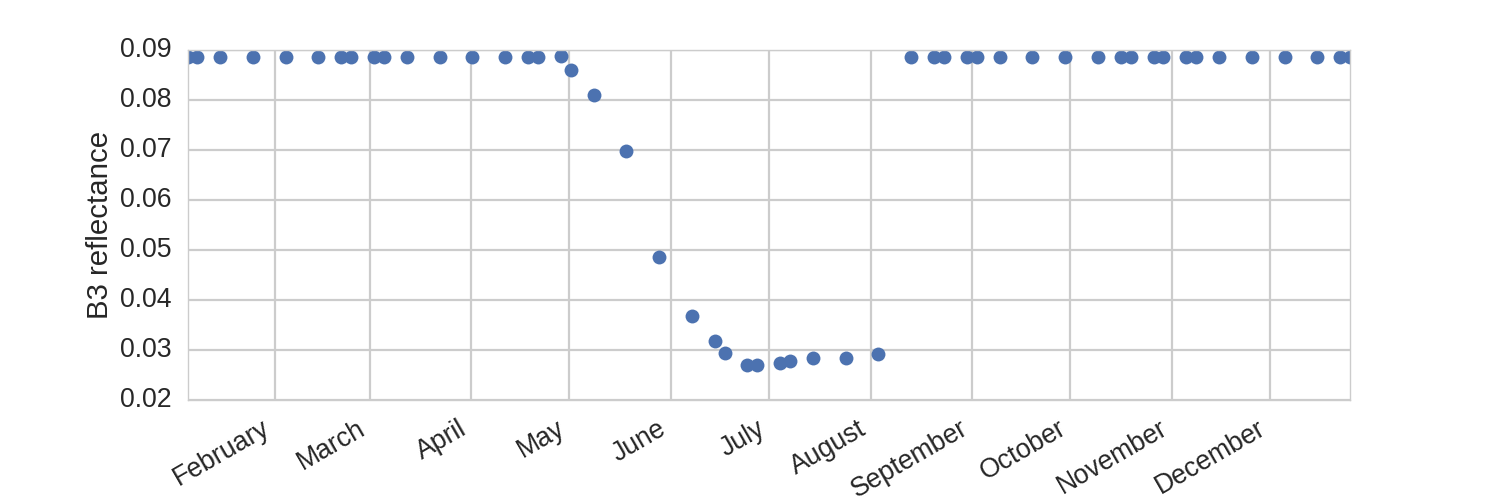
\includegraphics{B3.png}

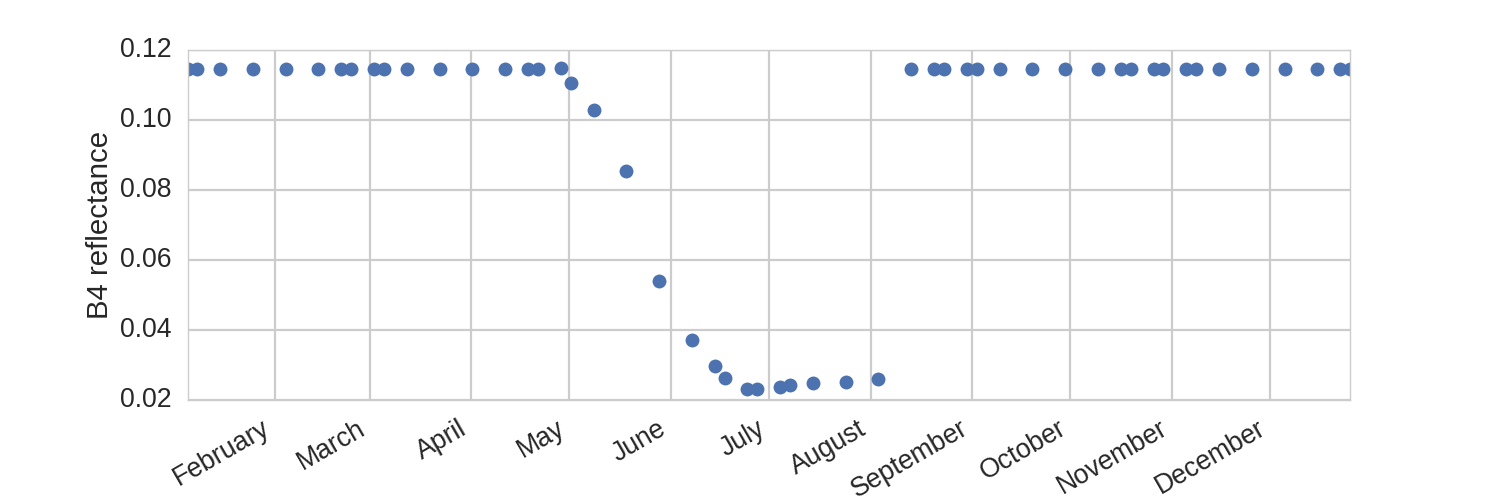
\includegraphics{B4.png}

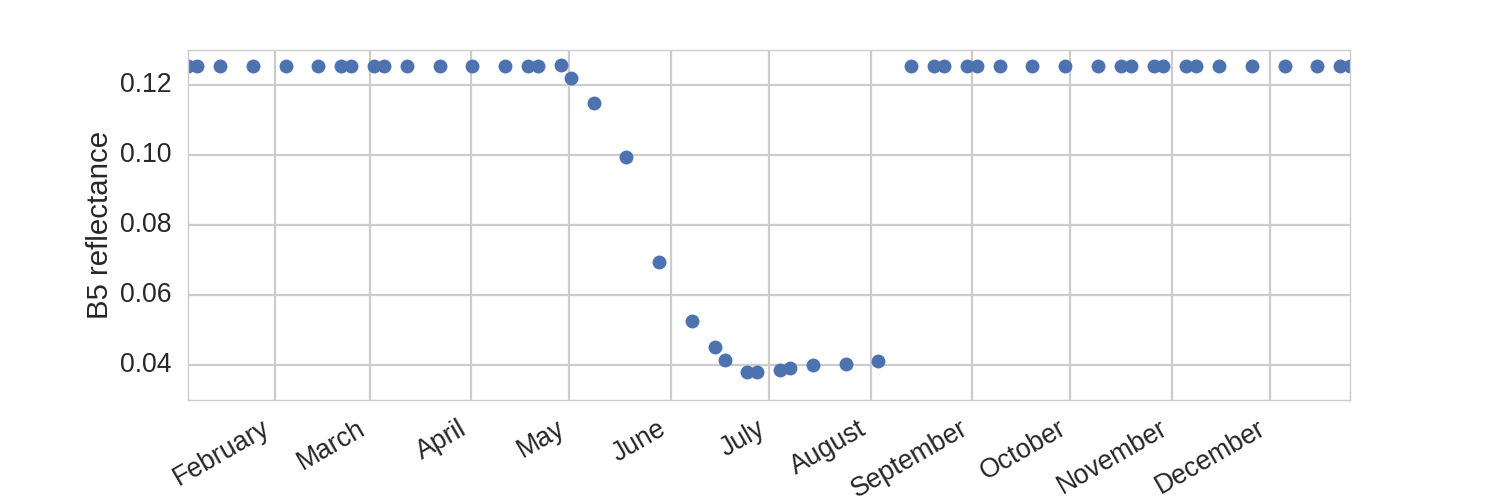
\includegraphics{B5.png}

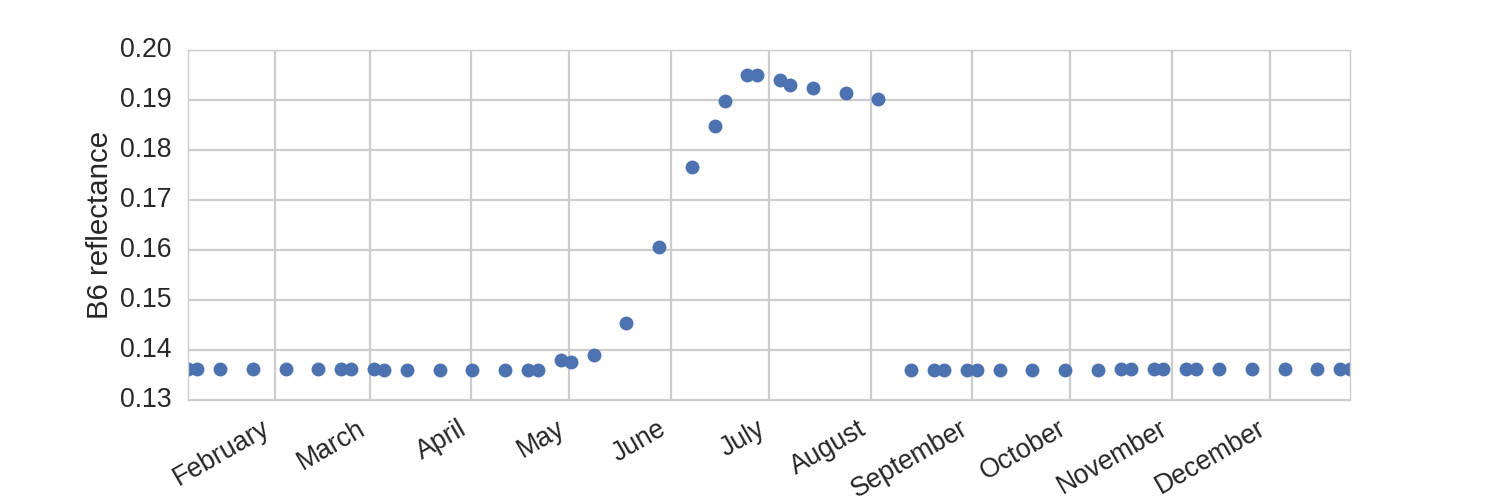
\includegraphics{B6.png}

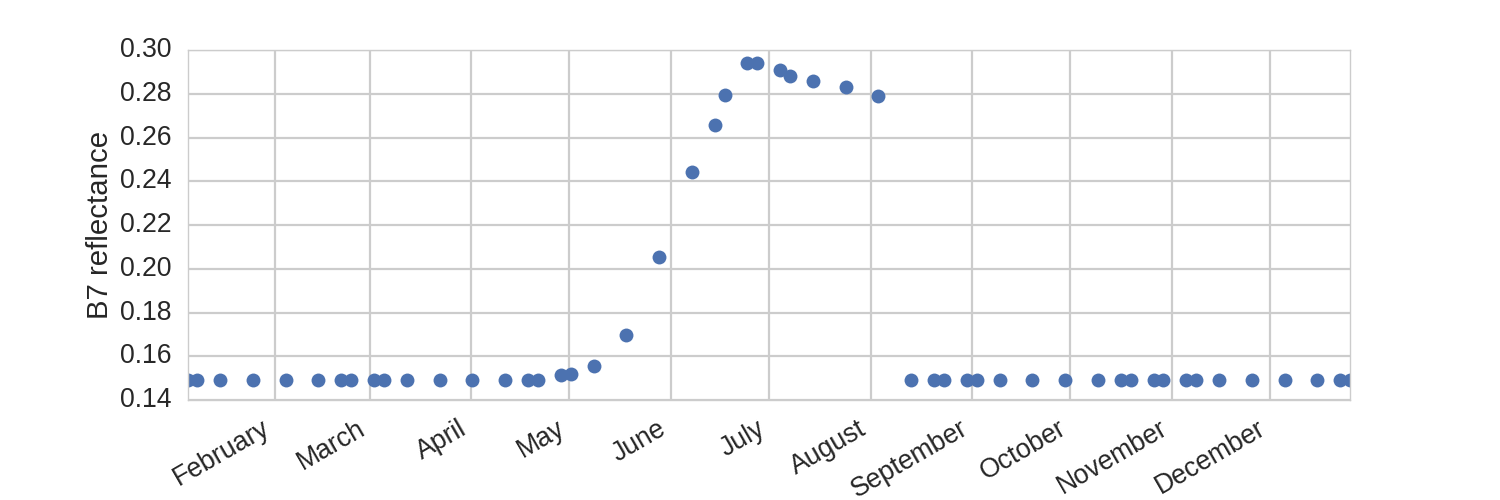
\includegraphics{B7.png}

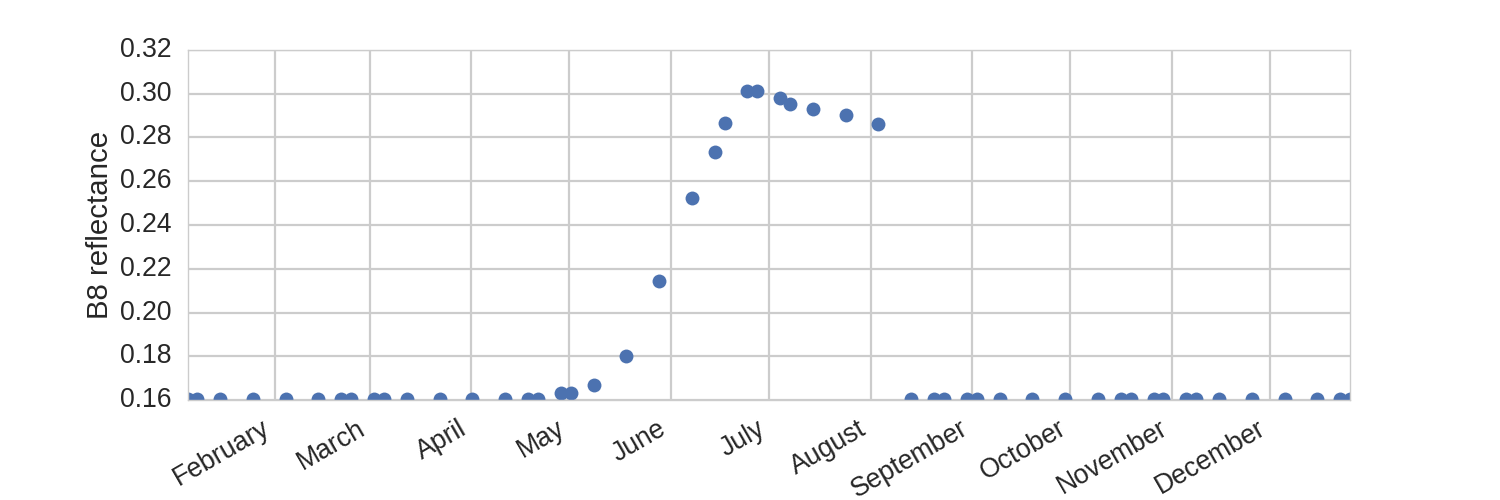
\includegraphics{B8.png}

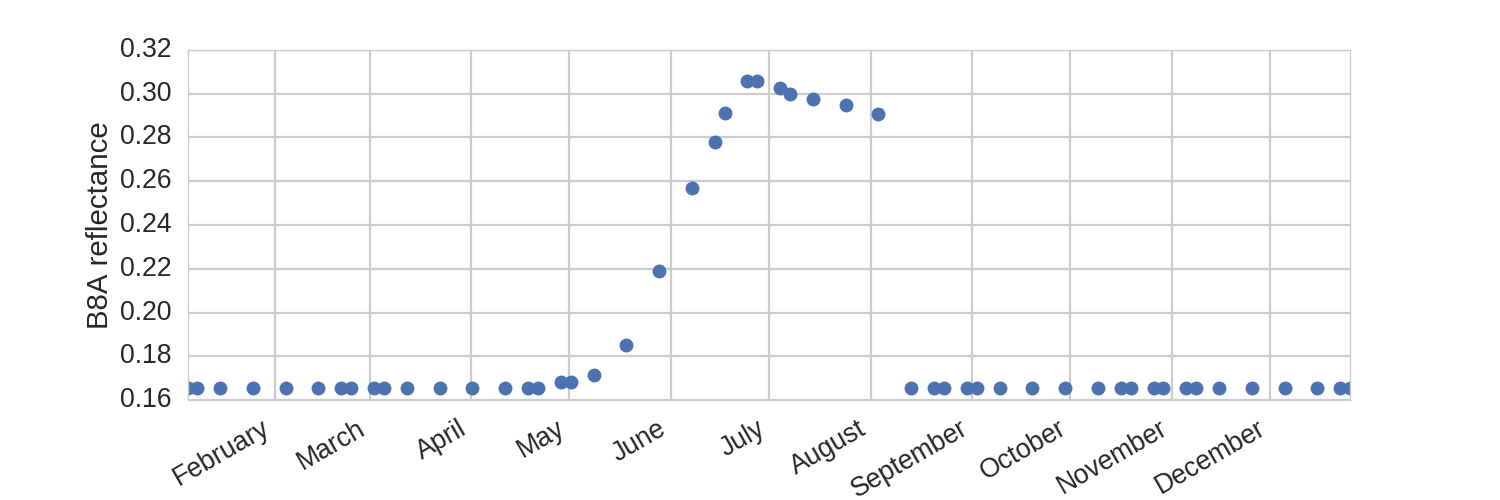
\includegraphics{B8A.png}

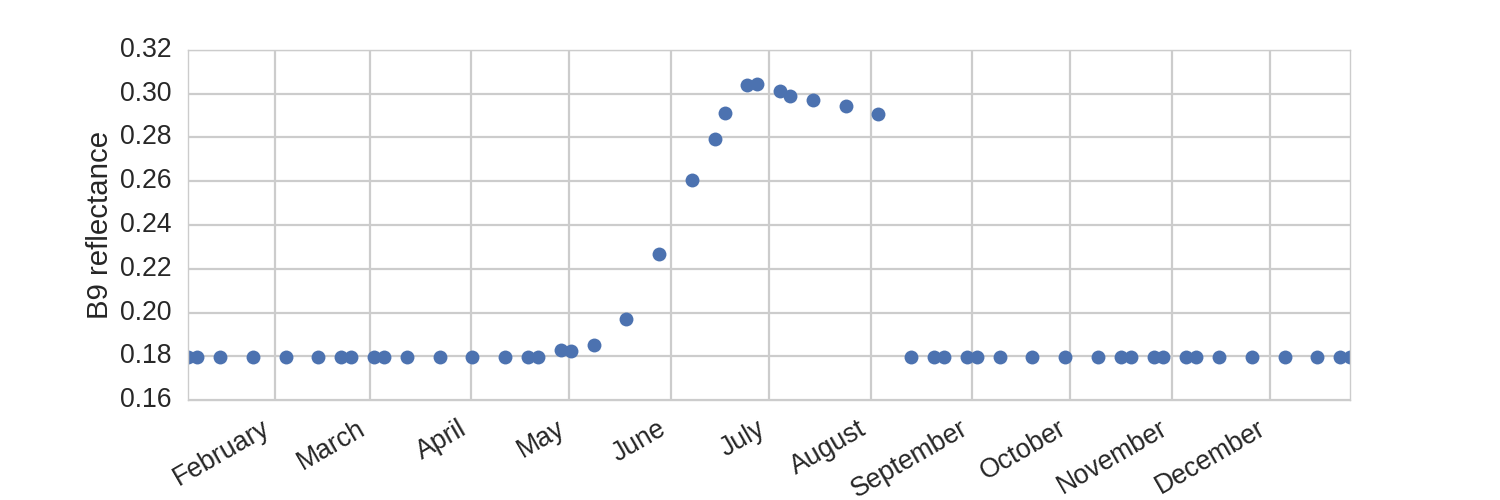
\includegraphics{B9.png}

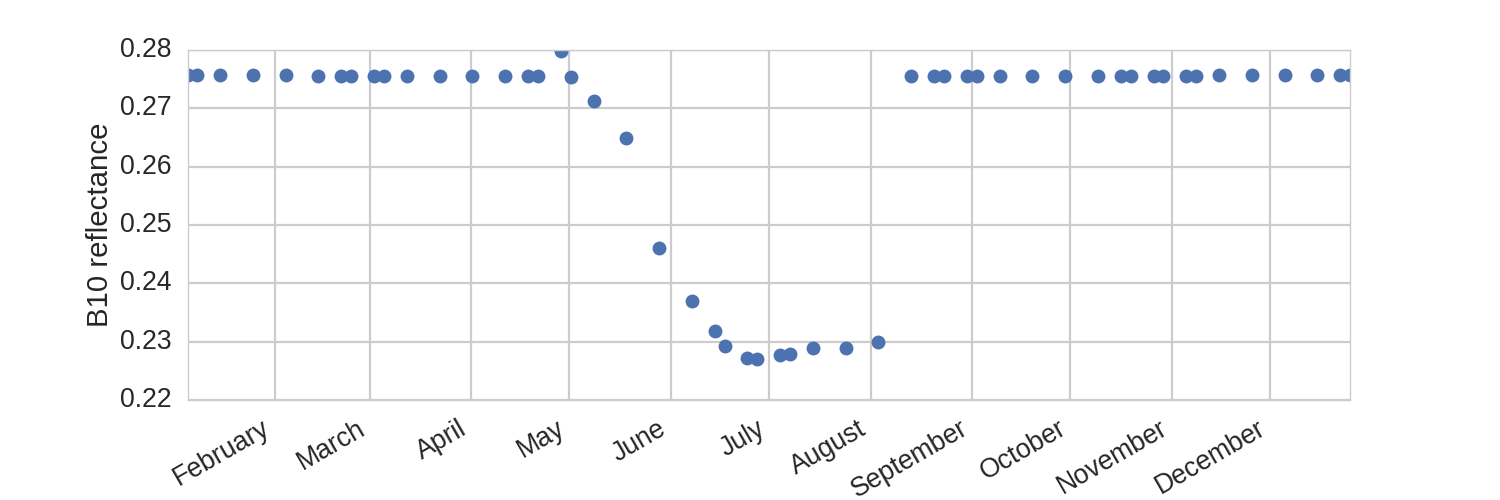
\includegraphics{B10.png}

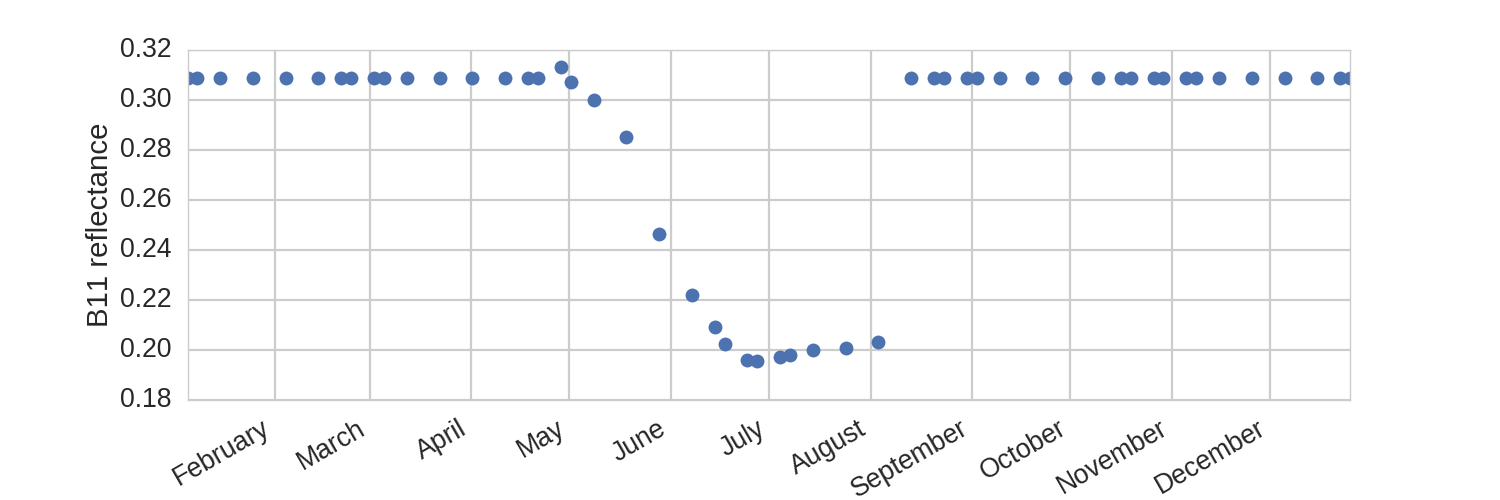
\includegraphics{B11.png}

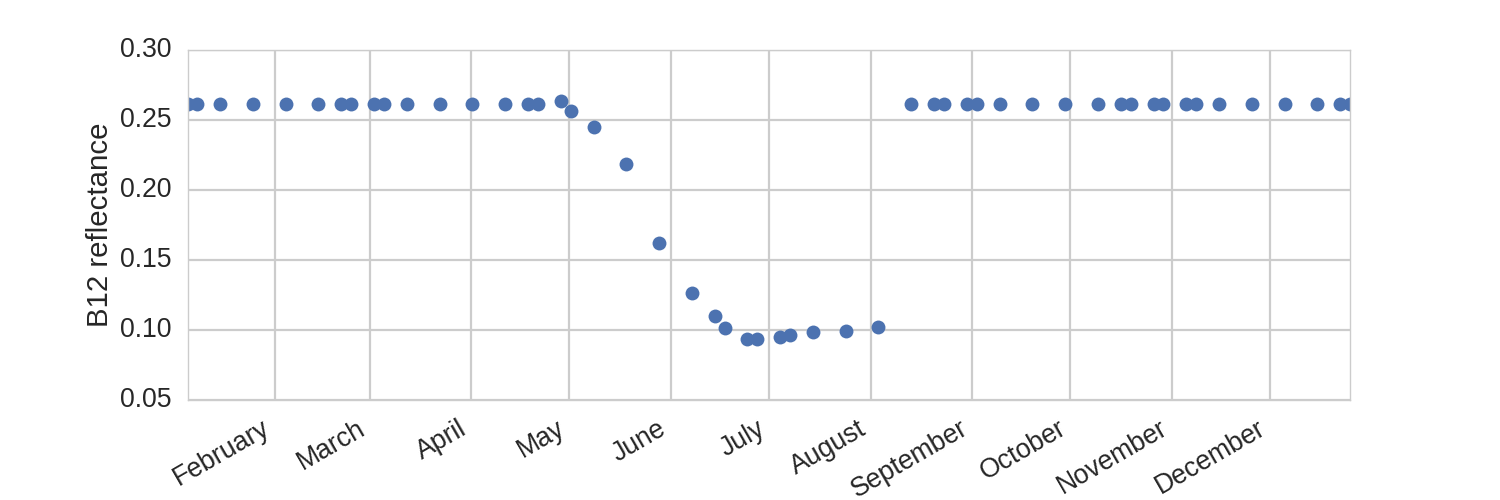
\includegraphics{B12.png}


\section{sentinel\_simulator}
\label{source/modules::doc}\label{source/modules:sentinel-simulator}

\subsection{sentinel\_simulator package}
\label{source/sentinel_simulator:sentinel-simulator-package}\label{source/sentinel_simulator::doc}

\subsubsection{Subpackages}
\label{source/sentinel_simulator:subpackages}

\paragraph{sentinel\_simulator.jules package}
\label{source/sentinel_simulator.jules:sentinel-simulator-jules-package}\label{source/sentinel_simulator.jules::doc}

\subparagraph{Submodules}
\label{source/sentinel_simulator.jules:submodules}

\subparagraph{sentinel\_simulator.jules.py\_importNML module}
\label{source/sentinel_simulator.jules:module-sentinel_simulator.jules.py_importNML}\label{source/sentinel_simulator.jules:sentinel-simulator-jules-py-importnml-module}\index{sentinel\_simulator.jules.py\_importNML (module)}\index{importJulesNML() (in module sentinel\_simulator.jules.py\_importNML)}

\begin{fulllineitems}
\phantomsection\label{source/sentinel_simulator.jules:sentinel_simulator.jules.py_importNML.importJulesNML}\pysiglinewithargsret{\code{sentinel\_simulator.jules.py\_importNML.}\bfcode{importJulesNML}}{\emph{nml}}{}
Parse a JULES nml file and write it in the style used for the
julesNML class.
\begin{quote}\begin{description}
\item[{Parameters}] \leavevmode
\textbf{nml} (\emph{str.}) -- JULES NML file name.

\item[{Returns}] \leavevmode
None

\end{description}\end{quote}

\end{fulllineitems}



\subparagraph{sentinel\_simulator.jules.py\_jules module}
\label{source/sentinel_simulator.jules:module-sentinel_simulator.jules.py_jules}\label{source/sentinel_simulator.jules:sentinel-simulator-jules-py-jules-module}\index{sentinel\_simulator.jules.py\_jules (module)}\index{crop\_run() (in module sentinel\_simulator.jules.py\_jules)}

\begin{fulllineitems}
\phantomsection\label{source/sentinel_simulator.jules:sentinel_simulator.jules.py_jules.crop_run}\pysiglinewithargsret{\code{sentinel\_simulator.jules.py\_jules.}\bfcode{crop\_run}}{\emph{sow\_date=110}, \emph{b=6.631}, \emph{smwilt=0.1866}, \emph{neff=0.00057}}{}
Function that runs JULES with crop model turned on and given user defined parameters at Wallerfing site. Output is
saved in folder and file specified within function.
\begin{quote}\begin{description}
\item[{Parameters}] \leavevmode\begin{itemize}
\item {} 
\textbf{sow\_date} (\emph{int.}) -- Sow date, between 90 and 150.

\item {} 
\textbf{b} (\emph{float.}) -- Brooks-Corey exponent factor.

\item {} 
\textbf{smwilt} (\emph{float.}) -- Soil moisture wilting point.

\item {} 
\textbf{neff} (\emph{float.}) -- Nitrogen use efficiency of crop (Vcmax).

\end{itemize}

\item[{Returns}] \leavevmode
`Done' to notify used JULES run has finished.

\item[{Return type}] \leavevmode
str

\end{description}\end{quote}

\end{fulllineitems}

\index{jules (class in sentinel\_simulator.jules.py\_jules)}

\begin{fulllineitems}
\phantomsection\label{source/sentinel_simulator.jules:sentinel_simulator.jules.py_jules.jules}\pysiglinewithargsret{\strong{class }\code{sentinel\_simulator.jules.py\_jules.}\bfcode{jules}}{\emph{jules\_exe='/home/if910917/jules/models/jules4.8/build/bin/jules.exe'}}{}
Bases: {\hyperref[source/sentinel_simulator.jules:sentinel_simulator.jules.py_jules.julesAllNML]{\code{sentinel\_simulator.jules.py\_jules.julesAllNML}}}

Class to run JULES.
\begin{quote}\begin{description}
\item[{Parameters}] \leavevmode
\textbf{jules\_exe} (\emph{str}) -- location of JULES executable.

\end{description}\end{quote}

\begin{notice}{note}{Note:}
You must have JULES installed on local system with a version of 4.8 or higher.
\end{notice}
\index{runJules() (sentinel\_simulator.jules.py\_jules.jules method)}

\begin{fulllineitems}
\phantomsection\label{source/sentinel_simulator.jules:sentinel_simulator.jules.py_jules.jules.runJules}\pysiglinewithargsret{\bfcode{runJules}}{}{}
Write all NML files to disk.
Run JULES in a subprocess.
Check output for fatal errors.
\begin{quote}\begin{description}
\item[{Returns}] \leavevmode
stdout and stderr output from JULES model run.

\item[{Return type}] \leavevmode
str

\end{description}\end{quote}

\end{fulllineitems}


\end{fulllineitems}

\index{julesAllNML (class in sentinel\_simulator.jules.py\_jules)}

\begin{fulllineitems}
\phantomsection\label{source/sentinel_simulator.jules:sentinel_simulator.jules.py_jules.julesAllNML}\pysigline{\strong{class }\code{sentinel\_simulator.jules.py\_jules.}\bfcode{julesAllNML}}
This class is populated by the contents
of a module which contains templates
of all the required JULES namelist files
\index{writeNML() (sentinel\_simulator.jules.py\_jules.julesAllNML method)}

\begin{fulllineitems}
\phantomsection\label{source/sentinel_simulator.jules:sentinel_simulator.jules.py_jules.julesAllNML.writeNML}\pysiglinewithargsret{\bfcode{writeNML}}{}{}
\end{fulllineitems}


\end{fulllineitems}



\subparagraph{sentinel\_simulator.jules.py\_julesNML module}
\label{source/sentinel_simulator.jules:module-sentinel_simulator.jules.py_julesNML}\label{source/sentinel_simulator.jules:sentinel-simulator-jules-py-julesnml-module}\index{sentinel\_simulator.jules.py\_julesNML (module)}
This module holds JULES namelist files. 
It has been automatically generated.
\index{julesNML (class in sentinel\_simulator.jules.py\_julesNML)}

\begin{fulllineitems}
\phantomsection\label{source/sentinel_simulator.jules:sentinel_simulator.jules.py_julesNML.julesNML}\pysiglinewithargsret{\strong{class }\code{sentinel\_simulator.jules.py\_julesNML.}\bfcode{julesNML}}{\emph{template}, \emph{filename}}{}
This is the base class for storing
and writing JULES namelist files
\index{update() (sentinel\_simulator.jules.py\_julesNML.julesNML method)}

\begin{fulllineitems}
\phantomsection\label{source/sentinel_simulator.jules:sentinel_simulator.jules.py_julesNML.julesNML.update}\pysiglinewithargsret{\bfcode{update}}{\emph{template}}{}
\end{fulllineitems}

\index{write() (sentinel\_simulator.jules.py\_julesNML.julesNML method)}

\begin{fulllineitems}
\phantomsection\label{source/sentinel_simulator.jules:sentinel_simulator.jules.py_julesNML.julesNML.write}\pysiglinewithargsret{\bfcode{write}}{}{}
\end{fulllineitems}


\end{fulllineitems}



\subparagraph{Module contents}
\label{source/sentinel_simulator.jules:module-sentinel_simulator.jules}\label{source/sentinel_simulator.jules:module-contents}\index{sentinel\_simulator.jules (module)}

\subsubsection{Submodules}
\label{source/sentinel_simulator:submodules}

\subsubsection{sentinel\_simulator.opticalCanopyRT module}
\label{source/sentinel_simulator:sentinel-simulator-opticalcanopyrt-module}\label{source/sentinel_simulator:module-sentinel_simulator.opticalCanopyRT}\index{sentinel\_simulator.opticalCanopyRT (module)}\index{canopyRTOptical() (in module sentinel\_simulator.opticalCanopyRT)}

\begin{fulllineitems}
\phantomsection\label{source/sentinel_simulator:sentinel_simulator.opticalCanopyRT.canopyRTOptical}\pysiglinewithargsret{\code{sentinel\_simulator.opticalCanopyRT.}\bfcode{canopyRTOptical}}{\emph{state}, \emph{geom}, \emph{resln=1.0}}{}
A python wrapper to the SemiDiscrete optical
canopy RT model of Nadine Gobron. Runs the
model for the the whole of its valid spectra
range at a resolution set by resln.
\begin{quote}\begin{description}
\item[{Parameters}] \leavevmode\begin{itemize}
\item {} 
\textbf{state} (\emph{instance}) -- Instance of the stateVector class.

\item {} 
\textbf{geom} (\emph{instance}) -- Instance of the sensorGeomety class.

\item {} 
\textbf{resln} (\emph{float}) -- the spectral resolution in nm {[}optional{]}.

\end{itemize}

\item[{Returns}] \leavevmode
Instance of the spectra class.

\item[{Return type}] \leavevmode
instance

\end{description}\end{quote}

\end{fulllineitems}



\subsubsection{sentinel\_simulator.satelliteGeometry module}
\label{source/sentinel_simulator:module-sentinel_simulator.satelliteGeometry}\label{source/sentinel_simulator:sentinel-simulator-satellitegeometry-module}\index{sentinel\_simulator.satelliteGeometry (module)}\index{getSentinel2Geometry() (in module sentinel\_simulator.satelliteGeometry)}

\begin{fulllineitems}
\phantomsection\label{source/sentinel_simulator:sentinel_simulator.satelliteGeometry.getSentinel2Geometry}\pysiglinewithargsret{\code{sentinel\_simulator.satelliteGeometry.}\bfcode{getSentinel2Geometry}}{\emph{startDateUTC}, \emph{lengthDays}, \emph{lat}, \emph{lon}, \emph{alt=0.0}, \emph{mission='Sentinel-2a'}, \emph{tleFile='../TLE/norad\_resource\_tle.txt'}}{}
Calculate approximate geometry for Sentinel overpasses.
Approximate because it assumes maximum satellite elevation
is the time at which target is imaged.
\begin{quote}\begin{description}
\item[{Parameters}] \leavevmode\begin{itemize}
\item {} 
\textbf{startDateUTC} (\emph{object}) -- a datetime object specifying when to start prediction.

\item {} 
\textbf{lengthDays} (\emph{int}) -- number of days over which to perform calculations.

\item {} 
\textbf{lat} (\emph{float}) -- latitude of target.

\item {} 
\textbf{lon} (\emph{float}) -- longitude of target.

\item {} 
\textbf{alt} (\emph{float}) -- altitude of target (in km).

\item {} 
\textbf{mission} (\emph{str}) -- mission name as in TLE file.

\item {} 
\textbf{tleFile} (\emph{str}) -- TLE file.

\end{itemize}

\item[{Returns}] \leavevmode
a python list containing instances of the sensorGeometry class arranged in date order.

\item[{Return type}] \leavevmode
list

\end{description}\end{quote}

\end{fulllineitems}

\index{sensorGeometry (class in sentinel\_simulator.satelliteGeometry)}

\begin{fulllineitems}
\phantomsection\label{source/sentinel_simulator:sentinel_simulator.satelliteGeometry.sensorGeometry}\pysigline{\strong{class }\code{sentinel\_simulator.satelliteGeometry.}\bfcode{sensorGeometry}}
Class to hold sun-sensor geometry information.
\index{printGeom() (sentinel\_simulator.satelliteGeometry.sensorGeometry method)}

\begin{fulllineitems}
\phantomsection\label{source/sentinel_simulator:sentinel_simulator.satelliteGeometry.sensorGeometry.printGeom}\pysiglinewithargsret{\bfcode{printGeom}}{}{}
Prints currently specified class attributes.

\end{fulllineitems}


\end{fulllineitems}



\subsubsection{sentinel\_simulator.spectra module}
\label{source/sentinel_simulator:module-sentinel_simulator.spectra}\label{source/sentinel_simulator:sentinel-simulator-spectra-module}\index{sentinel\_simulator.spectra (module)}\index{UnknownFileType}

\begin{fulllineitems}
\phantomsection\label{source/sentinel_simulator:sentinel_simulator.spectra.UnknownFileType}\pysigline{\strong{exception }\code{sentinel\_simulator.spectra.}\bfcode{UnknownFileType}}
Bases: \code{exceptions.Exception}

Exception class for unknown filetypes

\end{fulllineitems}

\index{convolve() (in module sentinel\_simulator.spectra)}

\begin{fulllineitems}
\phantomsection\label{source/sentinel_simulator:sentinel_simulator.spectra.convolve}\pysiglinewithargsret{\code{sentinel\_simulator.spectra.}\bfcode{convolve}}{\emph{s1orig}, \emph{s2orig}, \emph{resln=1.0}, \emph{s2norm=True}}{}
Convolve one spectra with another, for example
to apply a band pass, or a spectral response function.
\begin{quote}\begin{description}
\item[{Parameters}] \leavevmode\begin{itemize}
\item {} 
\textbf{s1orig} (\emph{object}) -- A spectra object.

\item {} 
\textbf{s2orig} (\emph{float}) -- A spectra object.

\item {} 
\textbf{resln} (\emph{float}) -- The spectral resolution to use.

\item {} 
\textbf{s2norm} (\emph{bool}) -- If True normalise the second spectra (e.g. to apply a spectra response function).

\end{itemize}

\item[{Returns}] \leavevmode
Convolved spectra.

\item[{Return type}] \leavevmode
object

\end{description}\end{quote}

\end{fulllineitems}

\index{sentinel2() (in module sentinel\_simulator.spectra)}

\begin{fulllineitems}
\phantomsection\label{source/sentinel_simulator:sentinel_simulator.spectra.sentinel2}\pysiglinewithargsret{\code{sentinel\_simulator.spectra.}\bfcode{sentinel2}}{\emph{s}, \emph{mission='a'}}{}
\end{fulllineitems}

\index{spectra (class in sentinel\_simulator.spectra)}

\begin{fulllineitems}
\phantomsection\label{source/sentinel_simulator:sentinel_simulator.spectra.spectra}\pysiglinewithargsret{\strong{class }\code{sentinel\_simulator.spectra.}\bfcode{spectra}}{\emph{fname=None}, \emph{ftype='SVC'}, \emph{wavlCol=0}, \emph{reflCol=1}, \emph{hdrLines=1}}{}
Bases: \code{object}

Spectra class for sentinel simulator.
\index{interpolate() (sentinel\_simulator.spectra.spectra method)}

\begin{fulllineitems}
\phantomsection\label{source/sentinel_simulator:sentinel_simulator.spectra.spectra.interpolate}\pysiglinewithargsret{\bfcode{interpolate}}{\emph{resltn=0.1}}{}
Interpolate spectra to the given resolution.
Overwites exisiting data.
\begin{quote}\begin{description}
\item[{Parameters}] \leavevmode
\textbf{resltn} (\emph{float}) -- resolution of the interpolation.

\end{description}\end{quote}

\end{fulllineitems}

\index{loadCSV() (sentinel\_simulator.spectra.spectra method)}

\begin{fulllineitems}
\phantomsection\label{source/sentinel_simulator:sentinel_simulator.spectra.spectra.loadCSV}\pysiglinewithargsret{\bfcode{loadCSV}}{\emph{f}, \emph{wavlCol=0}, \emph{reflCol=1}, \emph{hdrLines=1}}{}
Read in data from a standard CSV file object.
\begin{quote}\begin{description}
\item[{Parameters}] \leavevmode\begin{itemize}
\item {} 
\textbf{f} (\emph{file}) -- File object.

\item {} 
\textbf{wavlCol} (\emph{int}) -- Column containing wavelengths.

\item {} 
\textbf{reflCol} (\emph{int}) -- Column containing reflectance data.

\item {} 
\textbf{hdrLines} (\emph{int}) -- Number of lines to skip at start of file.

\end{itemize}

\end{description}\end{quote}

\end{fulllineitems}

\index{loadSVCSig() (sentinel\_simulator.spectra.spectra method)}

\begin{fulllineitems}
\phantomsection\label{source/sentinel_simulator:sentinel_simulator.spectra.spectra.loadSVCSig}\pysiglinewithargsret{\bfcode{loadSVCSig}}{\emph{f}}{}
Read in data from an SVC .sig ascii file.
\begin{quote}\begin{description}
\item[{Parameters}] \leavevmode
\textbf{f} (\emph{file}) -- File object.

\end{description}\end{quote}

\end{fulllineitems}

\index{loadSpectra() (sentinel\_simulator.spectra.spectra method)}

\begin{fulllineitems}
\phantomsection\label{source/sentinel_simulator:sentinel_simulator.spectra.spectra.loadSpectra}\pysiglinewithargsret{\bfcode{loadSpectra}}{\emph{fname}, \emph{wavlCol=0}, \emph{reflCol=1}, \emph{hdrLines=1}}{}
Load in the spectra from a given file using a
method appropriate to the type of file.

\begin{notice}{note}{Note:}
Current supported formats are:

SVC - SCV .sig ascii file

CSV - standard ascii comma seperated values
\end{notice}
\begin{quote}\begin{description}
\item[{Parameters}] \leavevmode\begin{itemize}
\item {} 
\textbf{fname} (\emph{str}) -- Valid filename containing spectra.

\item {} 
\textbf{wavlCol} (\emph{int}) -- Column containing wavelengths.

\item {} 
\textbf{reflCol} (\emph{int}) -- Column containing reflectance data.

\item {} 
\textbf{hdrLines} (\emph{int}) -- Number of lines to skip at start of file.

\end{itemize}

\end{description}\end{quote}

\end{fulllineitems}

\index{trim() (sentinel\_simulator.spectra.spectra method)}

\begin{fulllineitems}
\phantomsection\label{source/sentinel_simulator:sentinel_simulator.spectra.spectra.trim}\pysiglinewithargsret{\bfcode{trim}}{\emph{wlmin}, \emph{wlmax}}{}
Trim the spectra so it is between two specified wavelengths. Destroys the original data.
\begin{quote}\begin{description}
\item[{Parameters}] \leavevmode\begin{itemize}
\item {} 
\textbf{wlmin} (\emph{float}) -- The lowest wavelength of the new spectra.

\item {} 
\textbf{wlmax} (\emph{float}) -- The highest wavelength of the new spectra.

\end{itemize}

\end{description}\end{quote}

\end{fulllineitems}


\end{fulllineitems}



\subsubsection{sentinel\_simulator.stateVector module}
\label{source/sentinel_simulator:module-sentinel_simulator.stateVector}\label{source/sentinel_simulator:sentinel-simulator-statevector-module}\index{sentinel\_simulator.stateVector (module)}\index{get\_jules\_state() (in module sentinel\_simulator.stateVector)}

\begin{fulllineitems}
\phantomsection\label{source/sentinel_simulator:sentinel_simulator.stateVector.get_jules_state}\pysiglinewithargsret{\code{sentinel\_simulator.stateVector.}\bfcode{get\_jules\_state}}{\emph{date\_utc}, \emph{nc\_file='jules/output/wallerfing\_79\_12.3\_hourly.nc'}}{}
Function that returns a stateVector instance for a given time.
:param date\_utc: datetime object of when to extract JULES output.
:type date\_utc: object
:param nc\_file: JULES output file from which to extract data.
:type nc\_file: str
:return: Instance of stateVector class.
:rtype: instance

\end{fulllineitems}

\index{nearest() (in module sentinel\_simulator.stateVector)}

\begin{fulllineitems}
\phantomsection\label{source/sentinel_simulator:sentinel_simulator.stateVector.nearest}\pysiglinewithargsret{\code{sentinel\_simulator.stateVector.}\bfcode{nearest}}{\emph{items}, \emph{pivot}}{}
\end{fulllineitems}

\index{read() (in module sentinel\_simulator.stateVector)}

\begin{fulllineitems}
\phantomsection\label{source/sentinel_simulator:sentinel_simulator.stateVector.read}\pysiglinewithargsret{\code{sentinel\_simulator.stateVector.}\bfcode{read}}{\emph{file\_format='jules'}, \emph{file\_str=None}, \emph{year=None}}{}
Reads output data to a dictionary of state vectors indexed by time.

\begin{notice}{note}{Note:}
This function requires sub-functions capable of reading specified file format.
\end{notice}
\begin{quote}\begin{description}
\item[{Parameters}] \leavevmode\begin{itemize}
\item {} 
\textbf{file\_format} -- format of output to read.

\item {} 
\textbf{file\_str} (\emph{str}) -- location of file.

\item {} 
\textbf{year} (\emph{int}) -- year of data to extract, if equal to None whole time series extracted

\end{itemize}

\item[{Returns}] \leavevmode
state dictionary.

\item[{Return type}] \leavevmode
dict

\end{description}\end{quote}

\end{fulllineitems}

\index{read\_jules() (in module sentinel\_simulator.stateVector)}

\begin{fulllineitems}
\phantomsection\label{source/sentinel_simulator:sentinel_simulator.stateVector.read_jules}\pysiglinewithargsret{\code{sentinel\_simulator.stateVector.}\bfcode{read\_jules}}{\emph{nc\_file=None}, \emph{year=None}}{}
Reads jules output from netCDF file and writes it to a dictionary indexed by date.
\begin{quote}\begin{description}
\item[{Parameters}] \leavevmode\begin{itemize}
\item {} 
\textbf{nc\_file} (\emph{str}) -- location of nc\_file.

\item {} 
\textbf{year} (\emph{int}) -- year of data to extract, if equal to None whole time series extracted.

\end{itemize}

\item[{Returns}] \leavevmode
state dictionary.

\item[{Return type}] \leavevmode
dict

\end{description}\end{quote}

\end{fulllineitems}

\index{stateVector (class in sentinel\_simulator.stateVector)}

\begin{fulllineitems}
\phantomsection\label{source/sentinel_simulator:sentinel_simulator.stateVector.stateVector}\pysigline{\strong{class }\code{sentinel\_simulator.stateVector.}\bfcode{stateVector}}
Class to hold state vector data for optical
and microwave canopy RT models.

\end{fulllineitems}



\subsubsection{Module contents}
\label{source/sentinel_simulator:module-sentinel_simulator}\label{source/sentinel_simulator:module-contents}\index{sentinel\_simulator (module)}

\chapter{Indices and tables}
\label{index:indices-and-tables}\begin{itemize}
\item {} 
\emph{genindex}

\item {} 
\emph{modindex}

\item {} 
\emph{search}

\end{itemize}


\renewcommand{\indexname}{Python Module Index}
\begin{theindex}
\def\bigletter#1{{\Large\sffamily#1}\nopagebreak\vspace{1mm}}
\bigletter{s}
\item {\texttt{sentinel\_simulator}}, \pageref{source/sentinel_simulator:module-sentinel_simulator}
\item {\texttt{sentinel\_simulator.jules}}, \pageref{source/sentinel_simulator.jules:module-sentinel_simulator.jules}
\item {\texttt{sentinel\_simulator.jules.py\_importNML}}, \pageref{source/sentinel_simulator.jules:module-sentinel_simulator.jules.py_importNML}
\item {\texttt{sentinel\_simulator.jules.py\_jules}}, \pageref{source/sentinel_simulator.jules:module-sentinel_simulator.jules.py_jules}
\item {\texttt{sentinel\_simulator.jules.py\_julesNML}}, \pageref{source/sentinel_simulator.jules:module-sentinel_simulator.jules.py_julesNML}
\item {\texttt{sentinel\_simulator.opticalCanopyRT}}, \pageref{source/sentinel_simulator:module-sentinel_simulator.opticalCanopyRT}
\item {\texttt{sentinel\_simulator.satelliteGeometry}}, \pageref{source/sentinel_simulator:module-sentinel_simulator.satelliteGeometry}
\item {\texttt{sentinel\_simulator.spectra}}, \pageref{source/sentinel_simulator:module-sentinel_simulator.spectra}
\item {\texttt{sentinel\_simulator.stateVector}}, \pageref{source/sentinel_simulator:module-sentinel_simulator.stateVector}
\end{theindex}

\renewcommand{\indexname}{Index}
\printindex
\end{document}
